\documentclass[12pt]{article}
\usepackage{graphicx}
\usepackage{hyperref}
\usepackage{eso-pic} 
\usepackage{lipsum} 
\setlength{\parindent}{0em}
\setlength{\parskip}{1em}

\title{Rapport TP \\Sécurité et aide à la décision \\ \textbf{Jeux d'Infection} }
\author{TOURE Papa Samba Khary \\ Amadou Binta DIALLO \\ Erwan Phillipe MENSAH \\ Daouda TRAORE}
\date{}
\begin{document}
\maketitle

\AddToShipoutPicture*
    {\put(440,650){
\includegraphics[width=6cm,height=6cm]{logo.jpg}}}
\mbox{}
\vfill
L2 Informatique 2021-2022 Université Caen Basse-Normandie.
\newpage

\section{Présentation}

Ce compte rendu porte sur les expériences réalisées sur les algorithmes 
\textbf{\textit{Minmax}} et \textbf{\textit{Alpha-Beta}} dans le cadre du cours
\textbf{sécurité et aide à la décision}.

Ces deux algorithmes recursifs sont grandement utilisés dans les domaines de l'intelligence
artificielle, de la prise de décision, des statistiques et 
des théories de jeux afin de  trouver l'action optimale minimisant les pertes maximales.

Minmax visite tout l'arbre de jeux pour faire remonter à la racine la meilleur valeur
que l'on peut obtenir.

Alpha-Beta est une optimistation de  minimax réduisant grandement le temps de calcul
permettant ainsi de chercher plus vite et à une profondeur bien plus importante comme nous le 
verrons dans le graph suivant.
\newpage
\section{Expériences sur le nombre de noeuds visités en fonction 
de la profondeur}

\begin{figure}[ht!]
	\begin{center}
		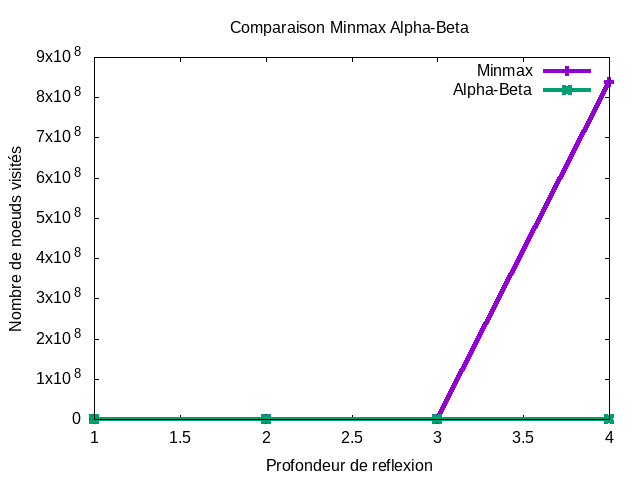
\includegraphics[width=1\textwidth]{fig3.png}
	\end{center}
	\caption{Comparaison du nombre de noeuds visités entre Minmax et Alpha-Beta}
	\label{fig1}
\end{figure}

\begin{figure}[ht!]
	\begin{center}
		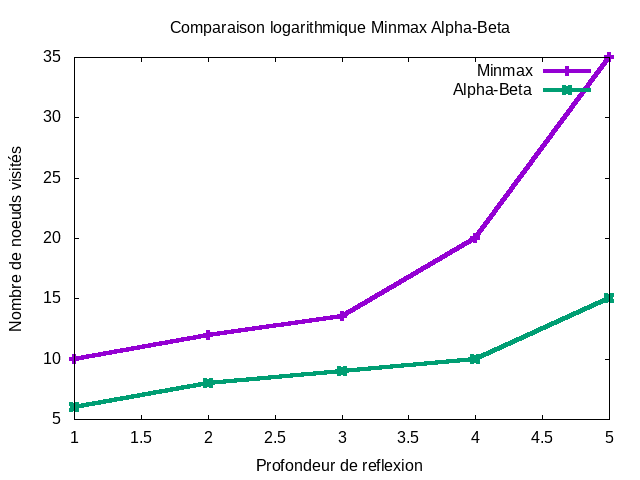
\includegraphics[width=1\textwidth]{fig1.png}
	\end{center}
	\caption{Répresentation logarithmique du nombre de neouds visités en fonction de la profondeur}
	\label{fig2}
\end{figure}

\newpage
\begin{table}[ht!]
    \centering
    
        \begin{tabular}{ |c |c |c|}
        \hline
        \textbf{Profondeur} & \textbf{Minmax} & \textbf{Alpha-Beta}\\
        \hline
        1 & 2330 & 580\\
        \hline
        2 & 120055 & 2660\\
        \hline
        3 & 568630 & 14252\\
        \hline
        4 & 838565053 & 17083\\ 
        \hline
        5 & ++185624468423 & 4423438\\
        \hline
        \end{tabular}
        \caption{Statistiques détaillés du nombre de noeuds visités}
        \label{tab1}
    
    \end{table}

\section{Conclusion}    
Comme nous le montre la figure \ref{fig1}  le nombre de  noeuds visités est considérablement
réduit avec Alpha-Béta et plus la profondeur est importante plus le rapport est grand.
En effet le nombre de noeuds visités par minimax croient de maniere exponentielle comme nous
pouvons le voir sur le tableau \ref{tab1}.

La comparaison logarithmique de la figure \ref{fig2} nous permet de voir une difference se former
dès le permier niveau de recherche et qui ne fait que s'accroître plus on s'enfonce dans les 
niveaux.


\end{document}